209. \begin{figure}[ht!]
\center{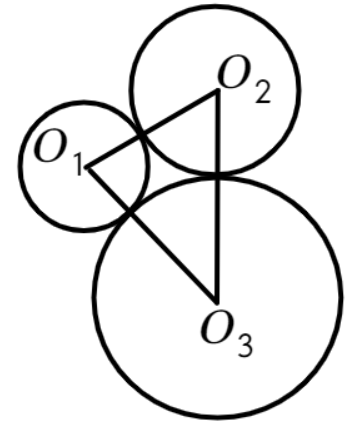
\includegraphics[scale=0.35]{g8-95.png}}
\end{figure}\\
Точки касания окружностей лежат на одной прямой с их центрами, поэтому $O_1O_2=5+6=11,\ O_1O_3=5+9=14,\ O_2O_3=6+9=15,\ p=\cfrac{11+14+15}{2}=20.$ Посчитаем его площадь двумя способами. С одной стороны, по формуле Герона она равна $\sqrt{20\cdot9\cdot6\cdot5}=30\sqrt{6},$ а с другой она равна $rp=20r.$ Значит, $r=30\sqrt{6}:20=\cfrac{3\sqrt{6}}{2}.$\\
